\documentclass[11pt]{article}
\usepackage[top=1.00in, bottom=1.0in, left=1.1in, right=1.1in]{geometry}
\usepackage{Sweave}
\renewcommand{\baselinestretch}{1.1}
\usepackage{graphicx}
\usepackage{natbib}
\usepackage{amsmath}
\usepackage{parskip}
\usepackage{todonotes}
\usepackage{xr-hyper}
\usepackage[utf8]{inputenc}
% \externaldocument{xxx}

\def\labelitemi{--}
\parindent=0pt

\begin{document}

\renewcommand{\refname}{\CHead{}}


\title{Do growing season length and growth relate? \\ And if not, why not? \\ And if we're not sure, why is that?}
\author{Team Grephon}
\date{\today}
\maketitle

The idea that longer growing seasons lead to increased plant growth is an intuitive tenet across multiple fields, including physiology (CITES), dendrochronology (CITES) and ecology. It is also a foundational assumption of most models of the future global carbon cycle (CITES). Most models project that future anthropogenic warming will be partly offset by increased carbon sequestration---primarily of temperate and boreal forests---as warming lengthens growing season (CITES), an assumption supported by a suite of ecosystem-scale studies (CITES). Yet recent work has called this assumption into question.

A suite of recent studies have suggested longer growing seasons do not lead to greater tree growth (CITES), with potentially large implications for future climate change. This research suggests limitations on plant growth mean forests will be limited sinks with increased warming. Such findings challenge decades of research that find growth does increase with longer seasons, from large-scale studies along natural elevational gradients (CITES) to small-scale studies of cell growth in lab settings (CITES) to previous studies of ecosystem fluxes with warming (CITES). Proposed mechanisms for the apparent disconnect are highly diverse, from previously unknown fundamental internal limits on plant growth (CITES) to effects of climate change itself, such as increased drought or temperatures too high for plant growth (CITES), as well as differences simply due to the metric of growth (GREEN KEENAN).

Here we review the connections between growing season length and plant growth across fields to identify the potential mechanisms that unite---and could disconnect---these processes. Our approach spans multiple fields to unify foundational studies with recent research related to anthropogenic warming. We find a pervasive disciplinary split between studies that limits our current ability to identify the underlying processes, and further highlight critical insights from physiology, community ecology, and life history theory that have been unexamined in recent work. Taken together, the current and past versions of fields studying connections between growing season length and growth appear primed to develop a holistic theory of when, where and how climate change may increase tree growth, with implications for both forecasts of future climate change and for fundamental science.

\emph{How warmer temperatures increase tree growth, or not}

Fundamentally, temperature limits biological processes and is a dominant controller of biological time. Temperatures that are too cool (often considered to be below 5C for temperate trees) and too warm (an area of active research but maybe 30-45C for trees???, but perhaps see a figure we'll add?) slow down biological processes to near-unobservably slow and eventually can lead to tissue death (CITES). Between the upper and lower limit biological processes underpinning growth generally accelerate such that warming can have a direct effect, effectively by accelerating biological time, up until the maximum rate (Fig. \ref{fig:concepbiotime}). This maximum rate means absolute time also matters to plant growth, which provides the mechanism through which longer growing seasons---extending absolute available time---can increase total plant growth. % Within this range, however, are most growing season temperatures as warm temperatures fundamentally define the growing season for many temperate plants. 
 
\newpage
\begin{figure}[h!]
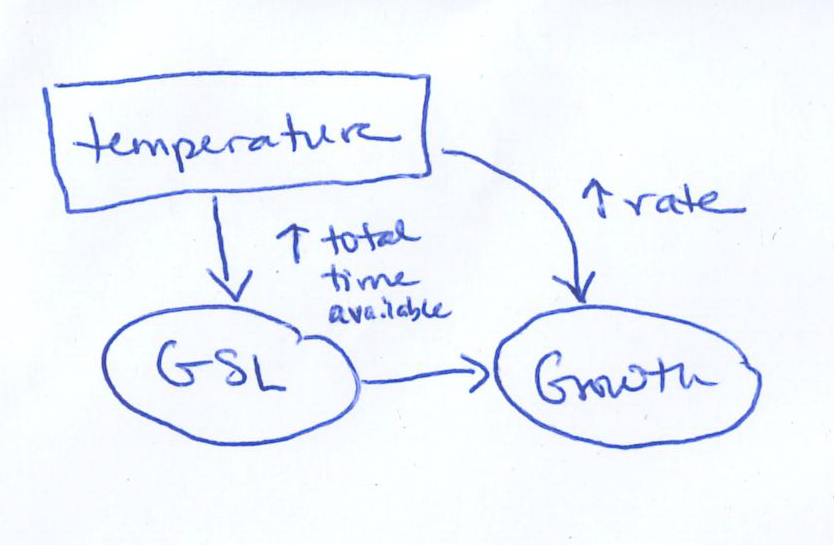
\includegraphics[width=0.5\textwidth]{..//figures/gsltogrowth/gsltogrowth_emw1a.png}
\caption{Idealized simplified version of the world, where resources (including water, N etc.) are abundant and temperatures are never too cool or too hot. In this world, temperature can increase growth directly (through increasing the speed of biological processes, up to some limit) and indirectly, but increasing the absolute available time for those processes to happen and lead to more growth.}
\label{fig:concepbiotime}
\end{figure}

i. Hypotheses for why GSL x growth is not found are not equally tested across fields: Constraint issues in provenance but not tree ring etc.
ii. Our premise is that some hypotheses for what is going may be tractably already answered by combining data across fields/methods
iii. And, you could go far by cross-field tweaking of what each field is doing

And somehow ... This is important!
i. Carbon storage and climate change
ii. Fundamental to physiology, species assembly

Studies that Green \& Keenan say no relationship:
% Fatichi et al. 2014 (opinion)
% Fatichi et al. 2019 (review)
% JIang et al 2020 (FACE or sinilar) 

Most global models of future warming assume increased anthropogenic carbon will be offset by increased carbon sequestration in forests as growing seasons lengthen.

The proposed mechanisms for this, however, are highly diverse---and most studies measure different aspects of growth across widely varying spatial and temporal scales. 

Yet the proposed mechanisms for this are highly diverse, as are the temporal and spatial scales of st


each with varying hypothesis for why. 

A positive link between longer growing seasons and increased carbon sequestration 

A suite of recent studies have called into question this fundamental assumption .... failed to find a link between longer seasons and increased tree growth

This assumption appeared well supported by several large-scale studies of ecosystem fluxes 



\newpage 
\emph{{\bf Warnings \& disclaimers:}
I flip between counting papers at the start to looking more at rows, so you were forewarned on that. }

\section{Old take home results from table}


Out of 38 papers (we have currently 62 rows of data) 20 found evidence for GS x growth (any which way) and  10 found evidence for our definition of GS x growth. Those papers with any evidence are:

\begin{Schunk}
\begin{Sinput}
> sort(unique(eviany$paper_id))
\end{Sinput}
\begin{Soutput}
 [1] "chen2000"                 "cuny2012"                
 [3] "delpierre2017"            "drew & downes 2018"      
 [5] "etzold2021"               "finzi2020"               
 [7] "francon2020"              "gao2022"                 
 [9] "grossiord2022"            "keenan et al 2014"       
[11] "mckown2016"               "michelot2012"            
[13] "moser2019"                "oddi2022"                
[15] "silvestro2023"            "soolananayakanahally2013"
[17] "vitasse2009"              "wheeler2016"             
[19] "zhu2021"                  "zohner2020"              
\end{Soutput}
\end{Schunk}

And those papers with evidence of our definition are (side query: how come Zhang2021 is here, but not showing up above?):
\begin{Schunk}
\begin{Sinput}
> sort(unique(eviour$paper_id))
\end{Sinput}
\begin{Soutput}
 [1] "cuny2012"           "delpierre2017"      "drew & downes 2018"
 [4] "grossiord2022"      "mckown2016"         "michelot2012"      
 [7] "oddi2022"           "silvestro2023"      "vitasse2009"       
[10] "zhang2021"         
\end{Soutput}
\end{Schunk}
and they cover both wood and plant vegetative studies:
\begin{Schunk}
\begin{Sinput}
> table(eviour$gsl)
\end{Sinput}
\begin{Soutput}
plant vegetative phenology          satellite derived 
                         6                          1 
            wood phenology 
                         5 
\end{Soutput}
\end{Schunk}
\newpage
Broadening beyond our definition includes studies where GS is not measured, or climate is used instead:
\begin{Schunk}
\begin{Sinput}
> table(eviany$gsl)
\end{Sinput}
\begin{Soutput}
              not measured plant vegetative phenology 
                         3                          9 
         satellite derived temperature or snow metric 
                         2                          4 
            wood phenology 
                         5 
\end{Soutput}
\end{Schunk}

\newpage
I have not checked whether that is different than random, but you can contrast that with the overall suite of GSL metrics and it looks representative to me on quick glance:
\begin{Schunk}
\begin{Sinput}
> table(d$gsl)
\end{Sinput}
\begin{Soutput}
                      date               not measured 
                         1                         14 
plant vegetative phenology          satellite derived 
                        21                          4 
temperature or snow metric             wood phenology 
                         9                         12 
\end{Soutput}
\end{Schunk}

They also cover a pretty wide diversity of growth metrics:
\begin{Schunk}
\begin{Sinput}
> table(eviany$growth) # any definition
\end{Sinput}
\begin{Soutput}
                      annual core cell production (number of cells) 
                                3                                 1 
        dendrometer/circumference                  ecosystem fluxes 
                                3                                 5 
                           height    intra-annual core (xylogeneis) 
                                5                                 3 
                   photosynthesis                  root:shoot ratio 
                                1                                 1 
                     stem density 
                                1 
\end{Soutput}
\begin{Sinput}
> table(eviour$growth) # our definition
\end{Sinput}
\begin{Soutput}
cell production (number of cells)         dendrometer/circumference 
                                1                                 2 
                 ecosystem fluxes                            height 
                                1                                 4 
   intra-annual core (xylogeneis)                    photosynthesis 
                                2                                 1 
                 root:shoot ratio 
                                1 
\end{Soutput}
\end{Schunk}

\newpage
Here's the full set of GS x growth that found it:
\begin{Schunk}
\begin{Sinput}
> table(eviany$gslxgrowth) # any definition
\end{Sinput}
\begin{Soutput}
                                 not measured x annual core 
                                                          1 
                            not measured x ecosystem fluxes 
                                                          1 
              not measured x intra-annual core (xylogeneis) 
                                                          1 
              plant vegetative phenology x ecosystem fluxes 
                                                          1 
                        plant vegetative phenology x height 
                                                          5 
plant vegetative phenology x intra-annual core (xylogeneis) 
                                                          1 
                plant vegetative phenology x photosynthesis 
                                                          1 
              plant vegetative phenology x root:shoot ratio 
                                                          1 
                       satellite derived x ecosystem fluxes 
                                                          2 
                   temperature or snow metric x annual core 
                                                          2 
              temperature or snow metric x ecosystem fluxes 
                                                          1 
                  temperature or snow metric x stem density 
                                                          1 
         wood phenology x cell production (number of cells) 
                                                          1 
                 wood phenology x dendrometer/circumference 
                                                          3 
            wood phenology x intra-annual core (xylogeneis) 
                                                          1 
\end{Soutput}
\begin{Sinput}
> table(eviour$gslxgrowth) # our definition
\end{Sinput}
\begin{Soutput}
               plant vegetative phenology x height 
                                                 4 
       plant vegetative phenology x photosynthesis 
                                                 1 
     plant vegetative phenology x root:shoot ratio 
                                                 1 
              satellite derived x ecosystem fluxes 
                                                 1 
wood phenology x cell production (number of cells) 
                                                 1 
        wood phenology x dendrometer/circumference 
                                                 2 
   wood phenology x intra-annual core (xylogeneis) 
                                                 2 
\end{Soutput}
\end{Schunk}

To contrast, here's what studies that did NOT find evidence looked like:
\begin{Schunk}
\begin{Sinput}
> table(noeviany$gslxgrowth) # any definition
\end{Sinput}
\begin{Soutput}
                                                 date x annual core 
                                                                  1 
                                    not measured x ecosystem fluxes 
                                                                  1 
                           plant vegetative phenology x annual core 
                                                                  3 
plant vegetative phenology x annual core (simulated to intraannual) 
                                                                  1 
                               plant vegetative phenology x biomass 
                                                                  1 
                                    satellite derived x annual core 
                                                                  1 
                           temperature or snow metric x annual core 
                                                                  1 
             temperature or snow metric x dendrometer/circumference 
                                                                  1 
                         wood phenology x dendrometer/circumference 
                                                                  3 
                    wood phenology x intra-annual core (xylogeneis) 
                                                                  2 
\end{Soutput}
\begin{Sinput}
> table(noeviour$gslxgrowth) # our definition
\end{Sinput}
\begin{Soutput}
    plant vegetative phenology x NDVI/greenness 
                                              1 
       plant vegetative phenology x annual core 
                                              3 
           plant vegetative phenology x biomass 
                                              1 
    plant vegetative phenology x photosynthesis 
                                              1 
             satellite derived x photosynthesis 
                                              1 
     wood phenology x dendrometer/circumference 
                                              1 
wood phenology x intra-annual core (xylogeneis) 
                                              1 
\end{Soutput}
\end{Schunk}

\section{Getting back to writing our paper}

\emph{Reminder of what we expected the table we worked on since April to help us with ...}
\begin{enumerate}
\item Section: Review three reasons for not growing 
\begin{enumerate} 
\item Overview paragraph of three reasons
\begin{enumerate} 
\item Measurement -- see box/figure  (include measurement only here or briefly so we move through it fast)
\item Resource limitation
\item Constraints
\end{enumerate}
\item Resource limitation, evidence for an against \todo{Table will help us with this}
\begin{enumerate}
\item Nutrients
\item Water
\item Is this more species-specific?
\end{enumerate}
\item Constraints, evidence for an against \todo{Table will help us with this}
\begin{enumerate}
\item Leaf life span
\item Budset stuff ... (Zohner, Sool.)
\item Evidence across species? Or which is species-specific
\end{enumerate}
\end{enumerate}
\item What do do next (The future! Is there a framework to our future directions? It would be nice if we found one) \todo{This needs a total overhaul after the table; figure out the section headers}
\end{enumerate}

\vspace{5ex}
So, we hoped these studies would help with the prevalence of evidence for external and endogenous factors. I haven't got as far on this (and we did not consistently enter whether growth or GSL or both was limiting) but here's a quick look at the 27 papers that found evidence of external factors and 14 that found evidence of endogenous (in contrast to 9 papers that looked but did not find evidence of external or 20 endogenous factors).

For those that did, they looked at these GSL metrics:
\begin{Schunk}
\begin{Sinput}
> table(exoyes$gsl)
\end{Sinput}
\begin{Soutput}
                      date               not measured 
                         1                         11 
plant vegetative phenology          satellite derived 
                        18                          1 
temperature or snow metric             wood phenology 
                         7                          5 
\end{Soutput}
\begin{Sinput}
> table(endoyes$gsl)
\end{Sinput}
\begin{Soutput}
              not measured plant vegetative phenology 
                        10                         11 
         satellite derived temperature or snow metric 
                         1                          2 
            wood phenology 
                         4 
\end{Soutput}
\end{Schunk}
And specifically:
\begin{Schunk}
\begin{Sinput}
> table(exoyes$gs_metric_used)
\end{Sinput}
\begin{Soutput}
                                                                           end metric only 
                                                                                         8 
growing season index (GSI - from minimum temperature, photoperiod, and evaporative demand) 
                                                                                         2 
                                                                         start metric only 
                                                                                         8 
                                                                              start to end 
                                                                                        14 
                                                          start to end (I think for SFGCC) 
                                                                                         1 
                                                                             suitable days 
                                                                                         1 
                             time with growth estimated (from mar-may temperature records) 
                                                                                         1 
                                                                 time with growth observed 
                                                                                         2 
                                                                                    unsure 
                                                                                         2 
\end{Soutput}
\begin{Sinput}
> table(endoyes$gs_metric_used)
\end{Sinput}
\begin{Soutput}
                                                                           end metric only 
                                                                                         8 
growing season index (GSI - from minimum temperature, photoperiod, and evaporative demand) 
                                                                                         2 
                                                                                      none 
                                                                                         1 
                                                                         start metric only 
                                                                                         5 
                                                                              start to end 
                                                                                         9 
                                                                 time with growth observed 
                                                                                         1 
                                                                                    unsure 
                                                                                         2 
\end{Soutput}
\end{Schunk}
And these growth metrics (seems a bias towards annual core studies looking at external; we have 13 annual core results):
\begin{Schunk}
\begin{Sinput}
> table(exoyes$growth)
\end{Sinput}
\begin{Soutput}
                        NDVI/greenness                            annual core 
                                     2                                     10 
annual core (simulated to intraannual)                                biomass 
                                     1                                      2 
             dendrometer/circumference                       ecosystem fluxes 
                                     3                                     10 
                                height         intra-annual core (xylogeneis) 
                                     5                                      3 
                        photosynthesis                       root:shoot ratio 
                                     6                                      1 
                          stem density 
                                     1 
\end{Soutput}
\begin{Sinput}
> table(endoyes$growth) 
\end{Sinput}
\begin{Soutput}
           NDVI/greenness               annual core                   biomass 
                        1                         1                         2 
dendrometer/circumference          ecosystem fluxes          growth anomalies 
                        4                        10                         1 
                   height            photosynthesis          root:shoot ratio 
                        4                         5                         1 
\end{Soutput}
\end{Schunk}

\section{Next steps}
\begin{enumerate}
\item How to finalize the table cleaning?
\begin{enumerate}
\item I would prefer this all documented over github than being done over email
\item Not sure how to resolve Richardson study
\item And there are likely more ....
\end{enumerate}
\item How do we want to analyze the table?
\begin{enumerate}
\item One idea is to break out what parts of the paper people are working on and then they do their own analysis -- but built off one set of shared cleaning code or such.
\item Work on analysis using the table is centralized in one person
\end{enumerate}
\item Do we want to make a figure that reviews the path diagram from GSL to growth and somehow summarizes what we have found?
\item Do we wan to re-analyze any of the studies that have the data but did not test our definition? (Dow2022, Finzi2020, Stridbeck2022, zani2020, chen1998, ren2019)
\item What else?
\end{enumerate}

\end{document}

\section{References}
\bibliography{/Users/Lizzie/Documents/git/bibtex/LizzieMainMinimal}
\bibliographystyle{/Users/Lizzie/Documents/git/bibtex/styles/besjournals.bst}
